\documentclass{beamer}
\usepackage{animate}
\beamertemplatenavigationsymbolsempty

\begin{document}
\begin{frame}

	\begin{figure}
	%\centering
	\only<1> {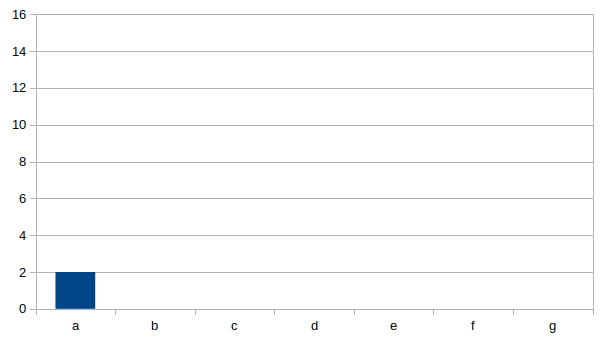
\includegraphics[scale=0.70]{a1}}
	\only<2> {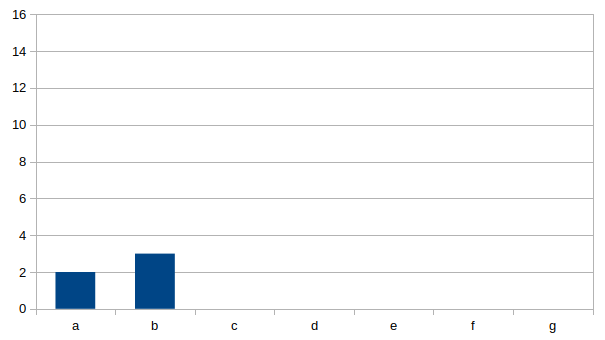
\includegraphics[scale=0.70]{a2}}
	\only<3> {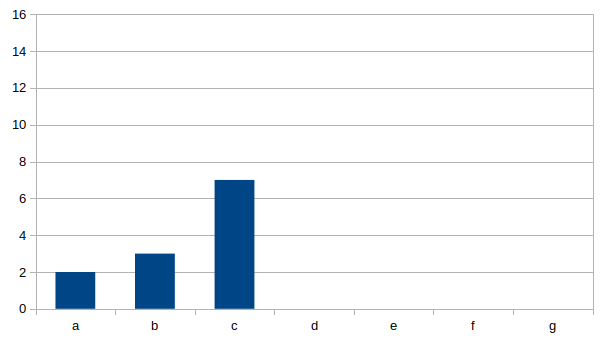
\includegraphics[scale=0.70]{a3}}
	\only<4> {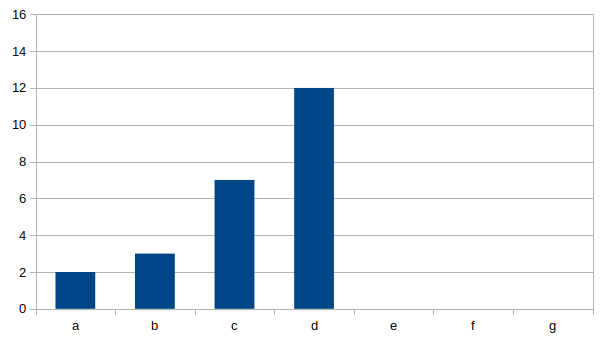
\includegraphics[scale=0.70]{a4}}
	\only<5> {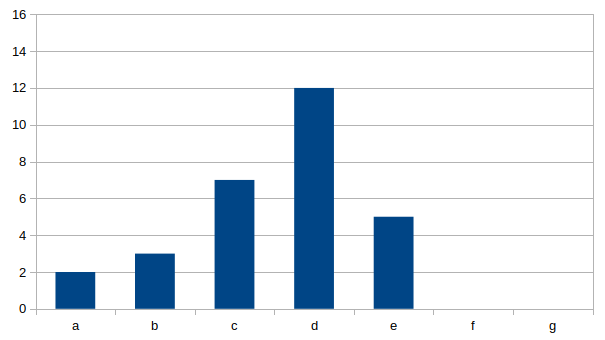
\includegraphics[scale=0.70]{a5}}
	\only<6> {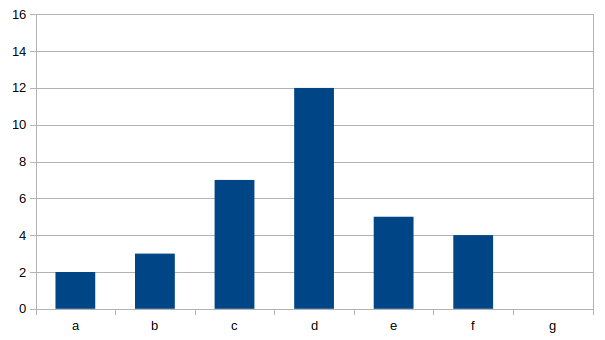
\includegraphics[scale=0.70]{a6}}
	\only<7> {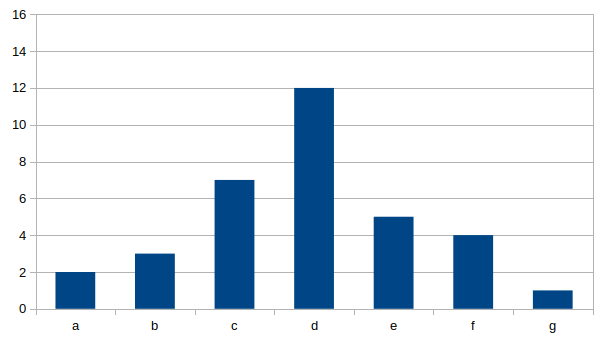
\includegraphics[scale=0.70]{a7}}
	\only<8> { }	
	% Tire a linha acima e veja a diferença no mupdf (último slide)
	\end{figure}

\end{frame}
\end{document}


